% \documentclass[english,edition=2025]{zpiday}
\documentclass[polish,edition=2025]{zpiday}

\usepackage{graphicx}
\usepackage{booktabs}
\usepackage{longtable}
\usepackage{amssymb}
\usepackage{subcaption}

\title{AI Present Finder}
\acronym{AIPF}
\supervisor{dr inż. Marcin Jodłowiec, Katedra Informatyki Stosowanej, Wydział Informatyki i Telekomunikacji}
\members{Bartosz Gotowski (DevOps, Profile Analysis) \and Dawid Chudzicki (Frontend, Fetch) \and Szymon Kowaliński (Chat, Gift Ideas) \and Marcin Dolatowski (Fetch, Reranking, Testy)}
\projectLogo{images/logo.png}


\begin{document}


\maketitle

\begin{abstract}
AI Present Finder to system rekomendacji prezentów łączący analizę profili publicznych (OSINT), konwersacyjny wywiad z użytkownikiem (chat), wieloźródłowe pobieranie ofert (OLX/Allegro/eBay/Amazon) oraz reranking oparty na AI, z natychmiastową prezentacją wyników w interfejsie (SSE). Architektura opiera się na mikroserwisach (NestJS, RabbitMQ, PostgreSQL) i froncie React. W środowisku produkcyjnym średni czas do pierwszych wyników wynosi ~7{,}7 min (464 s), asystent zadaje średnio 12 pytań, a lista produktów redukuje się z ok. 116 do ~70 pozycji po filtracji. Reranking z pełnym uzasadnieniem AI poprawia trafność (eliminacja niepasujących wyników). W~pilotażowej grupie testowej (11 opinii z 6 sesji) użytkownicy zadeklarowali średnio 80\% satysfakcji i 64\% trafności TOP‑1; wyniki wymagają walidacji na większej próbie. Projekt pokazuje, że połączenie social‑data + chat + multi‑fetch + reranking + SSE znacząco skraca czas wyboru i podnosi jakość rekomendacji.
\end{abstract}

\section{Wstęp}

\subsection{Problem: czasochłonność i nietrafione prezenty}

Wybór odpowiedniego prezentu to powszechne wyzwanie, które angażuje znaczne zasoby czasu i generuje stres. Według badań Consumer Reports~\cite{consumer-reports}, w sezonie świątecznym przeciętny Amerykanin poświęca \textbf{około 15 godzin} na zakupy prezentowe, przy czym kobiety spędzają na poszukiwaniach niemal dwukrotnie więcej czasu niż mężczyźni (20 vs 10 godzin). Podobną dysproporcję odnotowano w Wielkiej Brytanii: kobiety przeznaczają średnio 13 godzin na wybór prezentu dla partnera, mężczyźni — tylko 4 godziny.

Mimo poświęcania wielu godzin, \textbf{ponad 50\% konsumentów} co roku otrzymuje przynajmniej jeden prezent, który im się nie podoba~\cite{finder-gifts}. Przeciętna osoba dostaje około 2 niechciane upominki rocznie, co przekłada się na \textbf{9,5 miliarda dolarów} wydawanych globalnie na prezenty, których nikt nie chce lub nie używa — około 71 USD na osobę rocznie. Po świętach ok. 40\% konsumentów planuje zwrócić przynajmniej jeden otrzymany prezent.

\subsection{Frustracje użytkowników}

Badania konsumenckie wskazują na kluczowe bolączki:

\begin{itemize}
    \item \textbf{Brak pomysłu} — aż 88\% badanych deklaruje trudność z wymyśleniem, co kupić, szczególnie dla bliskich osób, które „wszystko już mają".
    \item \textbf{Presja społeczna} — około 40\% ludzi odczuwa presję związaną z wyborem odpowiedniego podarunku; wśród millenialsów odsetek ten sięga 60\%.
    \item \textbf{Stres i niepokój} — 58\% kupujących otwarcie stwierdza, że szukanie prezentów jest stresujące; 71\% doświadczyło tzw. \emph{gift anxiety} w ostatnim roku.
    \item \textbf{Paradoks wyboru} — 19\% wskazuje, że zbyt duży wybór produktów online utrudnia decyzję, a kolejne 19\% narzeka na trudności z filtrowaniem ofert.
    \item \textbf{Obawa przed porażką} — 55\% badanych ma w otoczeniu osobę, dla której bardzo trudno kupić prezent.
\end{itemize}

Co istotne, \textbf{77\% kupujących online} deklaruje frustrację przy zakupach prezentów w sieci, a wśród pokolenia Z i millenialsów odsetek ten przekracza 80\%. Aż 45\% konsumentów stwierdziło, że sklepy mogłyby najbardziej pomóc poprzez \textbf{podpowiedzi i inspiracje} ułatwiające znalezienie przemyślanego prezentu.

\subsection{Cel i zakres projektu}

Odpowiedzią na powyższe wyzwania jest \textbf{AI Present Finder} — system, który:

\begin{enumerate}
    \item \textbf{Skraca czas} — zamiast godzin poszukiwań, użytkownik otrzymuje trafne propozycje w kilka minut.
    \item \textbf{Zwiększa trafność} — wykorzystuje publiczne dane społecznościowe (Instagram/TikTok/X) oraz konwersacyjny wywiad AI do zbudowania profilu obdarowywanego.
    \item \textbf{Agreguje źródła} — przeszukuje równolegle OLX, Allegro, eBay i Amazon, eliminując potrzebę ręcznego przeglądania wielu serwisów.
    \item \textbf{Wyjaśnia decyzje} — reranking AI dostarcza pełne uzasadnienia, dlaczego dany produkt pasuje (lub nie) do profilu.
\end{enumerate}

\noindent\textbf{Kryteria sukcesu projektu:} (a)~czas do pierwszych wyników $<$10~min, (b)~subiektywna trafność rekomendacji $>$60\%, (c)~stabilność systemu produkcyjnego (0 awarii krytycznych), (d)~przejrzyste uzasadnienia AI dla każdej propozycji.

Zakres MVP obejmuje: zautomatyzowaną analizę profili publicznych (BrightData~\cite{brightdata}), chat (Gemini 2.5-flash~\cite{google-gemini}), generowanie pomysłów (GPT-4o~\cite{openai-api}), multi-source fetch, reranking (Gemini 2.5-flash-lite), realtime SSE~\cite{sse-spec} oraz OAuth+JWT i persystencję w PostgreSQL.

\section{Prace związane z tematem}

\subsection{Analiza konkurencji}

Na rynku istnieje kilka narzędzi wspomagających wybór prezentów. Tabela~\ref{tab:competition} zestawia ich kluczowe cechy z możliwościami AI Present Finder.

\begin{table}[h]
    \centering
    \caption{Porównanie z istniejącymi rozwiązaniami}
    \label{tab:competition}
    \begin{tabular}{lccccc}
        \toprule
        \textbf{Narzędzie} & \textbf{Social data} & \textbf{Wywiad AI} & \textbf{Multi-source} & \textbf{Reranking AI} & \textbf{Live SSE} \\
        \midrule
        DreamGift & -- & częściowo & -- & -- & -- \\
        GiftAssistant & -- & tak & -- & -- & -- \\
        Giftruly & -- & tak & -- & -- & -- \\
        IntelliGift & -- & częściowo & -- & -- & -- \\
        \textbf{AI Present Finder} & \checkmark & \checkmark & \checkmark & \checkmark & \checkmark \\
        \bottomrule
    \end{tabular}
\end{table}

Konkurencyjne rozwiązania opierają się głównie na wywiadzie z użytkownikiem, ale nie wykorzystują publicznych danych społecznościowych do wzbogacenia profilu obdarowywanego. Żadne z nich nie agreguje ofert z wielu serwisów e-commerce ani nie stosuje rerankingu z pełnym uzasadnieniem AI. AI Present Finder jako jedyny dostarcza wyniki w czasie rzeczywistym (SSE), co eliminuje oczekiwanie na pełne przetworzenie.

\subsection{Architektura systemu}

System oparty jest na architekturze mikroserwisowej~\cite{newman-microservices} (rys.~\ref{fig:c4container}). Każdy mikroserwis odpowiada za wydzieloną domenę i komunikuje się asynchronicznie przez RabbitMQ.

\begin{figure}[h]
    \centering
    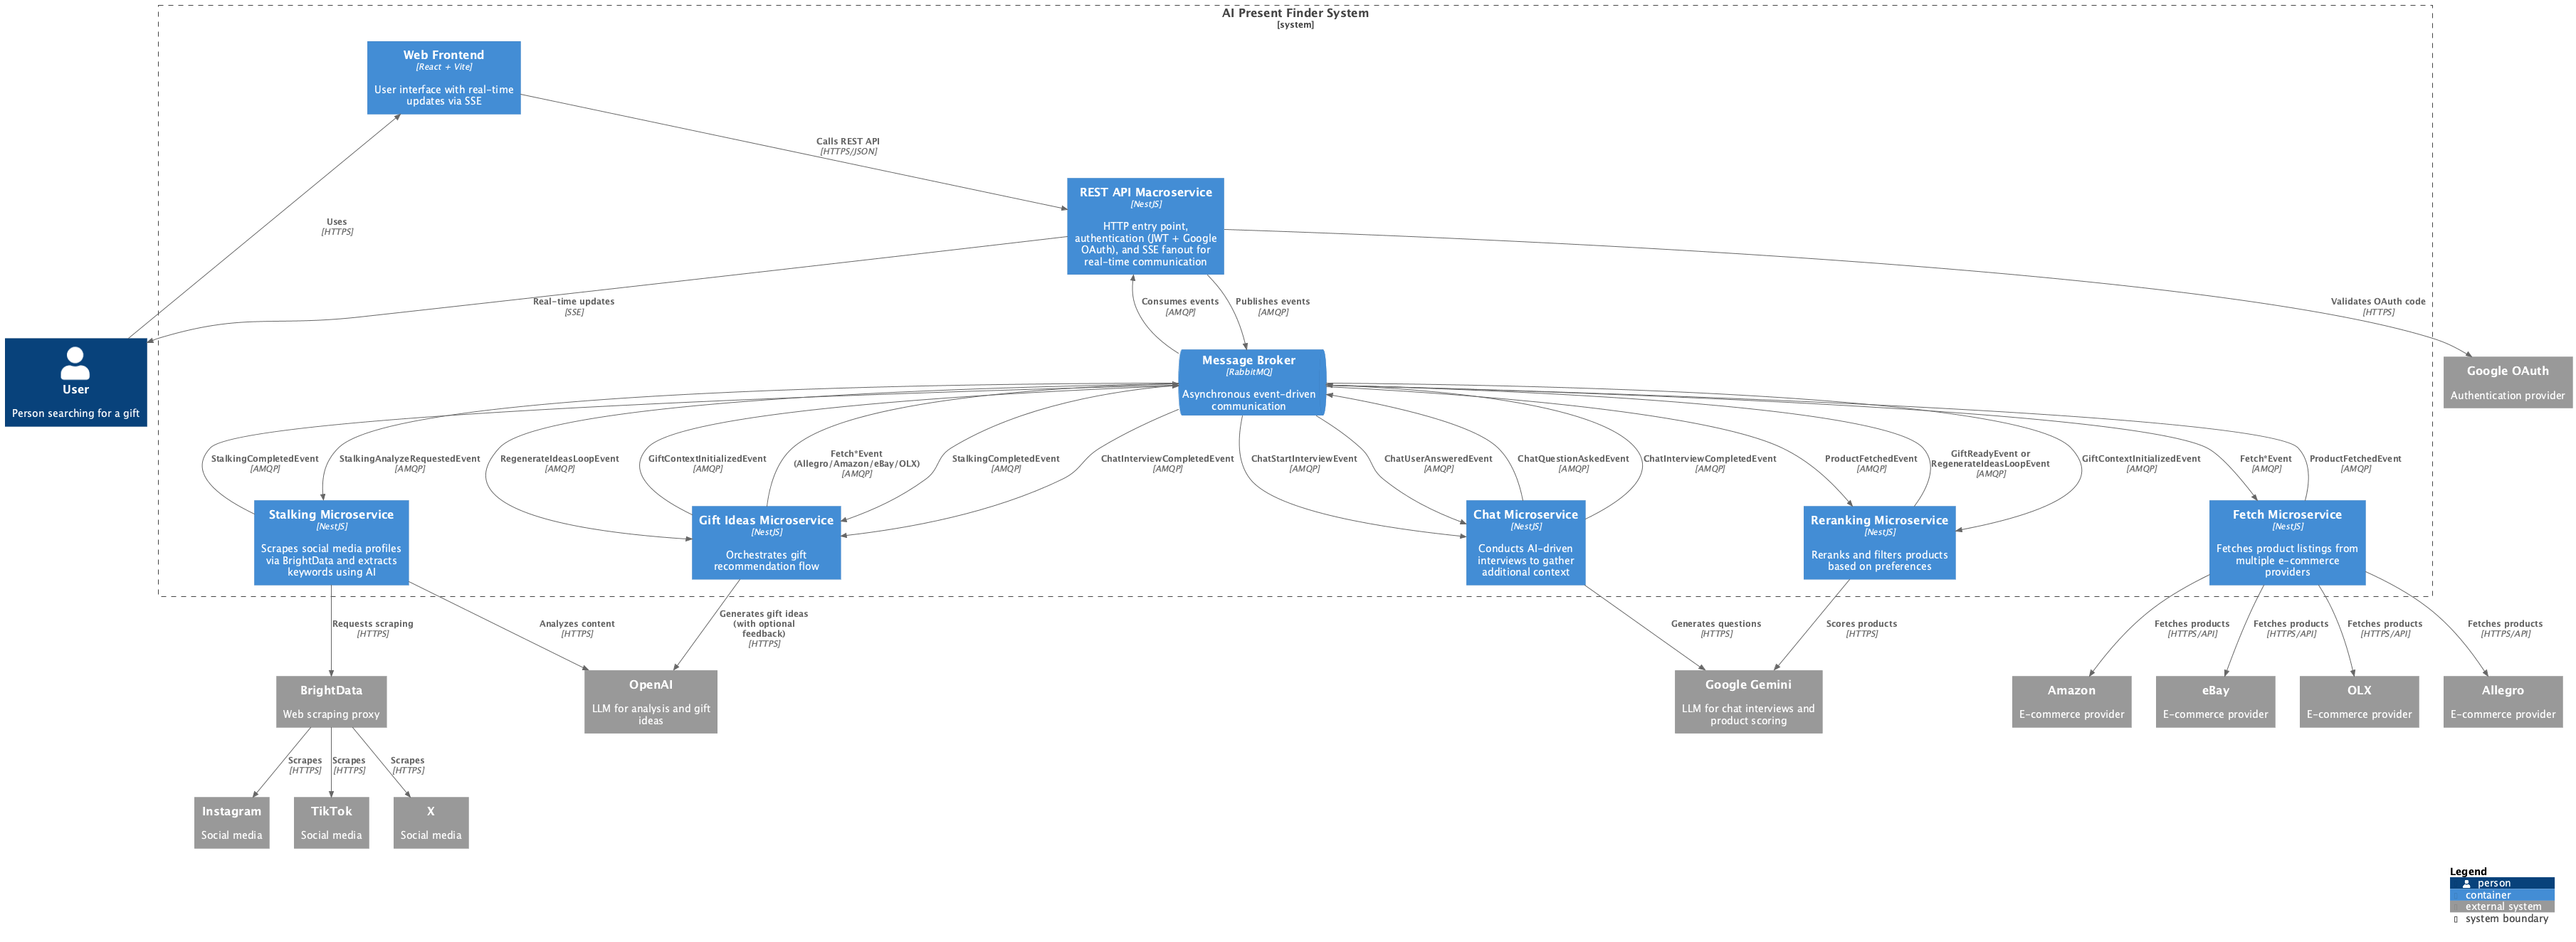
\includegraphics[width=0.95\linewidth]{images/C4_Container.png}
    \caption{Diagram kontenerów C4 — architektura AI Present Finder}
    \label{fig:c4container}
\end{figure}

Przepływ zdarzeń przebiega następująco: (1) użytkownik podaje linki do profili społecznościowych i inicjuje wyszukiwanie, (2) \texttt{profile-analysis-microservice} pobiera dane przez BrightData i ekstrahuje słowa kluczowe, (3) \texttt{chat-microservice} prowadzi wywiad doprecyzowujący, (4) \texttt{gift-ideas-microservice} generuje propozycje prezentów, (5) \texttt{fetch-microservice} (x4 instancje) pobiera oferty z OLX/Allegro/eBay/Amazon, (6) \texttt{reranking-microservice} ocenia i filtruje produkty, (7) wyniki strumieniowo trafiają do frontendu przez SSE.

\subsection{Stos technologiczny}

Tabela~\ref{tab:stack} przedstawia mikroserwisy i wykorzystywane modele AI.

\begin{table}[h]
    \centering
    \caption{Mikroserwisy i modele AI}
    \label{tab:stack}
    \begin{tabular}{lll}
        \toprule
        \textbf{Mikroserwis} & \textbf{Model AI} & \textbf{Zastosowanie} \\
        \midrule
        restapi-macroservice & -- & HTTP entry, OAuth, SSE fanout \\
        profile-analysis & OpenAI gpt-5-nano & Ekstrakcja słów kluczowych z profili \\
        chat-microservice & Google Gemini 2.5-flash & Wywiad konwersacyjny (tool-based) \\
        gift-ideas-microservice & OpenAI GPT-4o & Generowanie pomysłów na prezenty \\
        fetch-microservice (x4) & -- & Pobieranie ofert (OLX/Allegro/eBay/Amazon) \\
        reranking-microservice & Google Gemini 2.5-flash-lite & Scoring i ranking produktów \\
        \bottomrule
    \end{tabular}
\end{table}

Wszystkie serwisy wykorzystują NestJS 11~\cite{nestjs} z wzorcem CQRS~\cite{cqrs-pattern}, komunikację przez RabbitMQ~\cite{rabbitmq} (AMQP) oraz persystencję w PostgreSQL (TypeORM~\cite{typeorm}). Frontend w React + TanStack Router/Query odbiera zdarzenia przez Server-Sent Events. Integracja z modelami AI odbywa się przez Vercel AI SDK~\cite{vercel-ai-sdk}.

\section{Wyniki}
System wdrożono produkcyjnie na platformie Coolify (VPS 4 vCPU / 8 GB RAM). Architektura mikroserwisowa (NestJS 11 + CQRS, RabbitMQ, PostgreSQL) odpowiada diagramom C4 v0.2.0. Frontend w React wykorzystuje SSE do strumieniowej prezentacji postępów. Dane zebrano 30.11.2025 z baz \texttt{restapi\_service} oraz \texttt{reranking\_service}.

\subsection{Metryki produkcyjne}

Tabela~\ref{tab:metrics} przedstawia kluczowe wskaźniki wydajności i skali systemu.

\begin{table}[h]
    \centering
    \caption{Metryki produkcyjne (stan na 30.11.2025)}
    \label{tab:metrics}
    \begin{tabular}{ll}
        \toprule
        \textbf{Metryka} & \textbf{Wartość} \\
        \midrule
        Łączna liczba sesji (chatów) & 36 \\
        Łączna liczba wiadomości & 815 \\
        Łączna liczba listingów & 1321 \\
        \midrule
        Średni czas do pierwszych ofert & 464 s ($\approx$ 7{,}7 min) \\
        Średnia liczba pytań asystenta & 12 \\
        Średnia liczba listingów na chat & 70 \\
        Produkty/sesję (przed $\to$ po rerankingu) & 116 $\to$ $\sim$70 \\
        \midrule
        Rozkład providerów & OLX 99{,}3\%, Allegro 0{,}7\% \\
        Zużycie RAM (9 mikroserwisów) & $\sim$769 MB \\
        Koszt infrastruktury & $\sim$20--25 USD/mies. \\
        \bottomrule
    \end{tabular}
\end{table}

Dominacja OLX w rozkładzie providerów wynika z agresywnych limitów rate-limit na API Allegro oraz braku pełnej integracji z Amazon/eBay w wersji MVP. Kolejki RabbitMQ pozostają puste (0 oczekujących wiadomości), co świadczy o sprawnym przetwarzaniu zdarzeń przez mikroserwisy.

\begin{figure}[h]
    \centering
    \begin{subfigure}[b]{0.48\textwidth}
        \centering
        
\includegraphics[width=\textwidth]{screenshots/chat.png}
        \caption{Widok konwersacji z asystentem AI}
        \label{fig:chat}
    \end{subfigure}
    \hfill
    \begin{subfigure}[b]{0.48\textwidth}
        \centering
        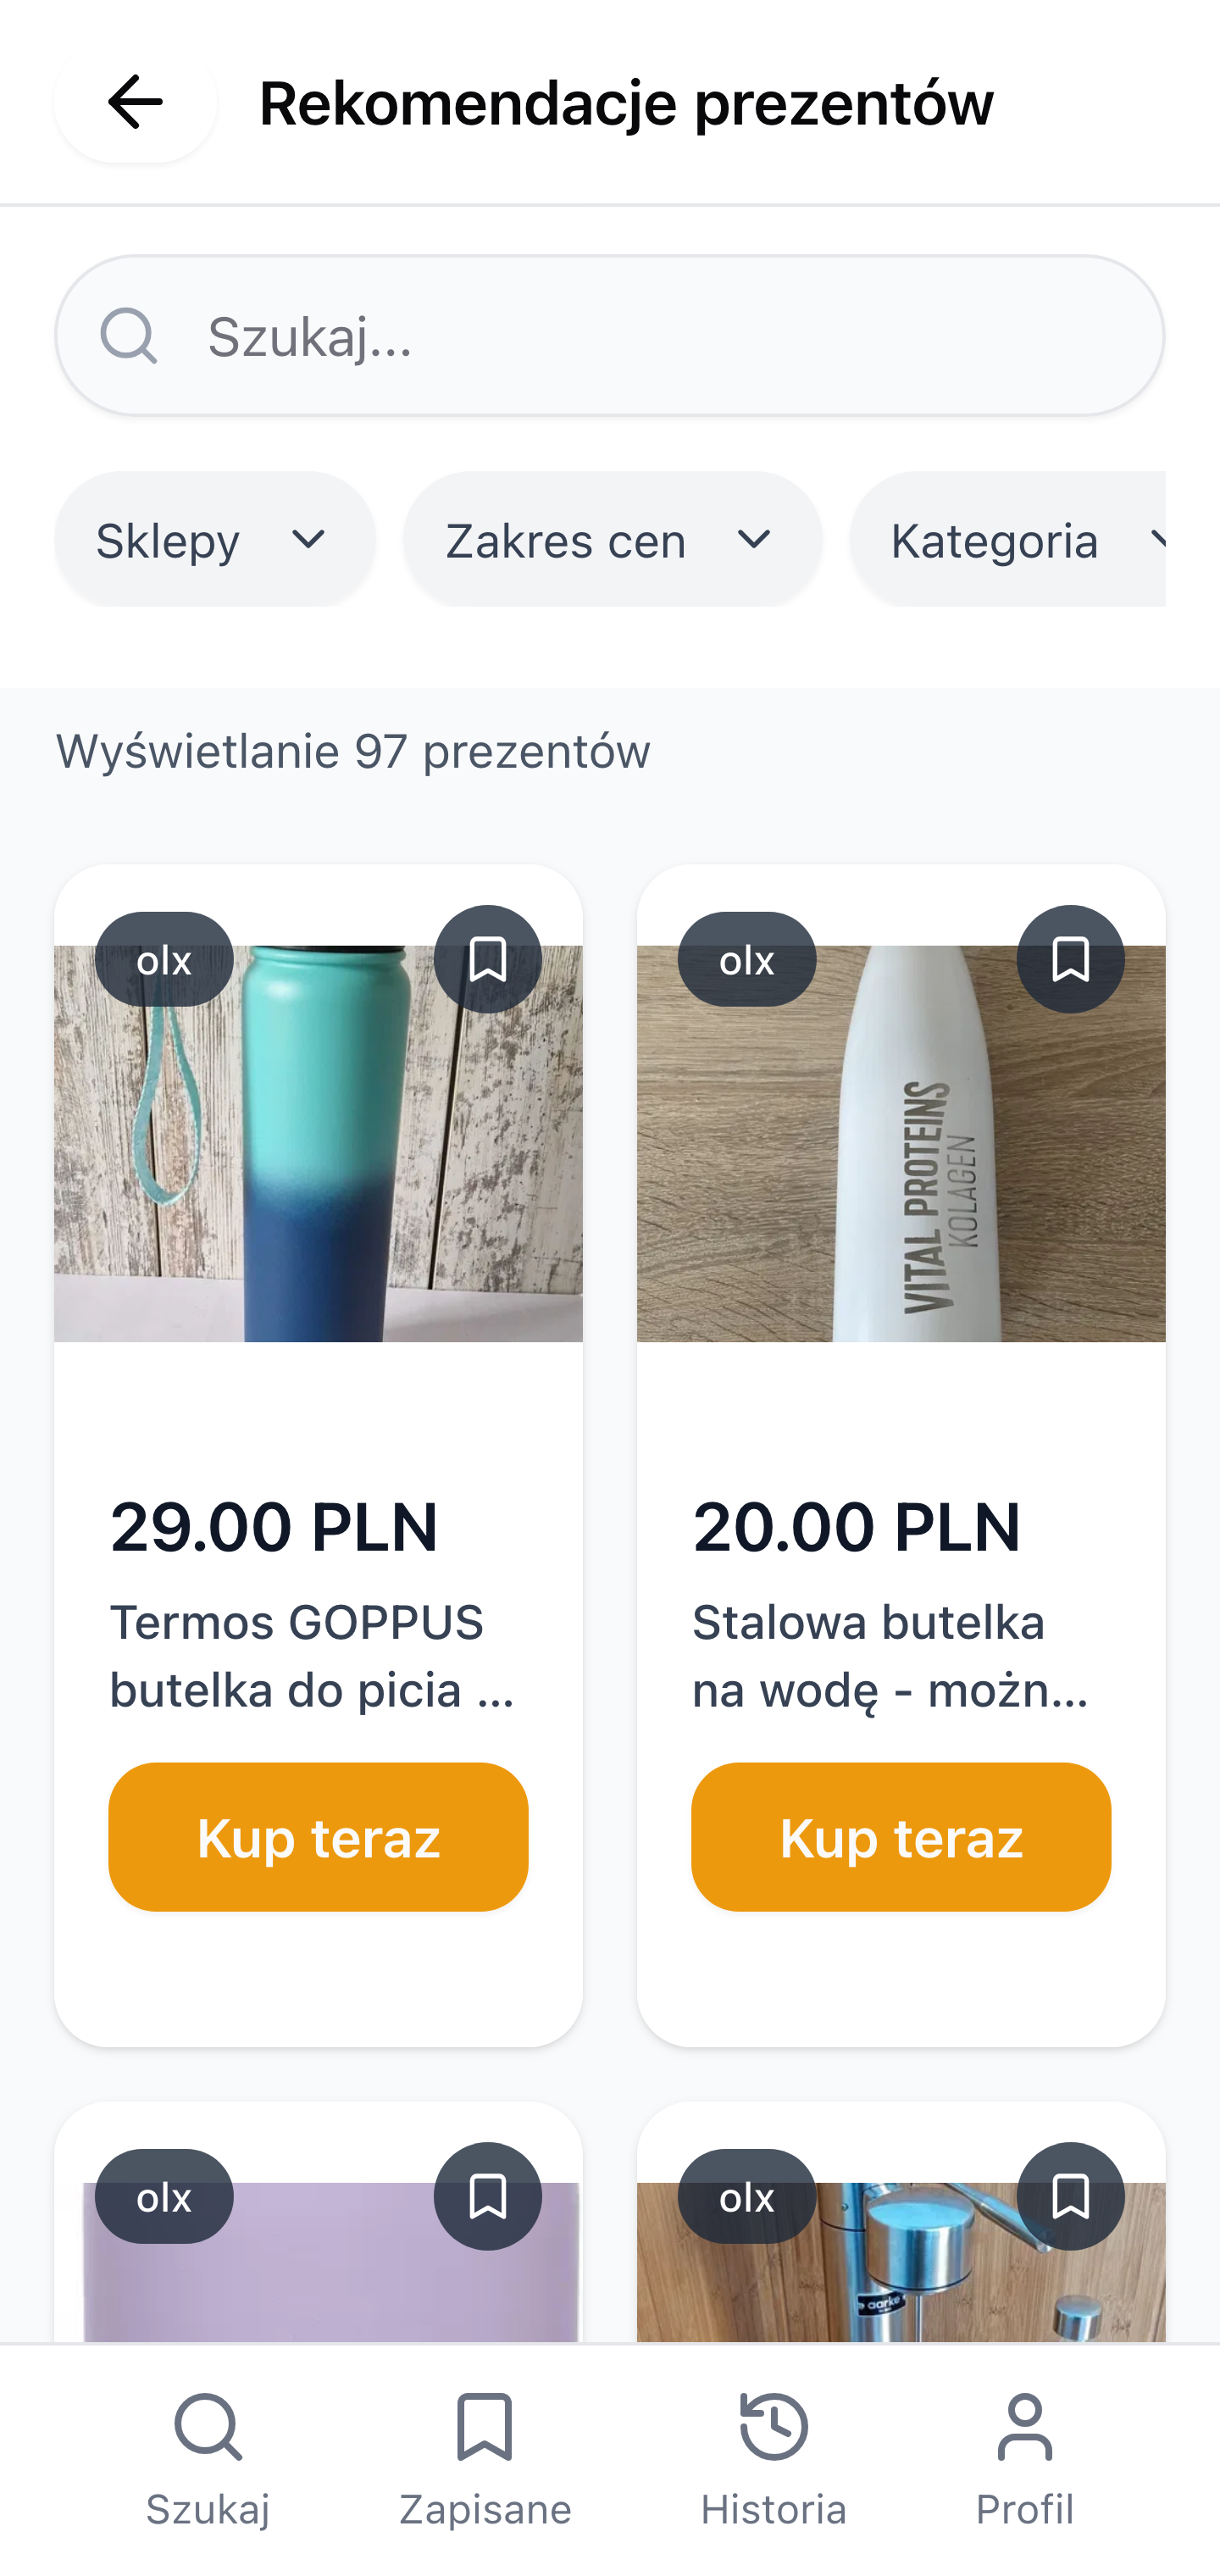
\includegraphics[width=\textwidth]{screenshots/rekomendacje_prezentów.png}
        \caption{Lista rekomendowanych produktów}
        \label{fig:recommendations}
    \end{subfigure}
    \caption{Interfejs użytkownika AI Present Finder: (a) wywiad prowadzony przez asystenta AI, (b) wyniki z uzasadnieniami i cenami.}
    \label{fig:ui-screenshots}
\end{figure}

\subsection{Studium przypadku: wywiad i rekomendacje}

Poniżej przedstawiono pełną transkrypcję przykładowej sesji (zanonimizowanej), w której użytkownik szukał prezentu świątecznego dla brata (26--35 lat, zainteresowany technologią). Wywiad trwał ok. 2 min 18 s i obejmował 14 pytań.

\begin{longtable}{p{0.12\linewidth}p{0.82\linewidth}}
\toprule
\textbf{Rola} & \textbf{Treść wiadomości} \\
\midrule
\endfirsthead
\toprule
\textbf{Rola} & \textbf{Treść wiadomości} \\
\midrule
\endhead
Asystent & Dla kogo szukasz prezentu z okazji święta? \\
Użytkownik & Dla członka rodziny (rodzice, rodzeństwo, dziadkowie). \\
Asystent & Kim dokładnie jest ta osoba z rodziny? \\
Użytkownik & To jest mój brat. \\
Asystent & W jakim przedziale wiekowym jest? \\
Użytkownik & 26--35 lat. \\
Asystent & Co robi w wolnym czasie? \\
Użytkownik & Interesuje się nowymi technologiami i gadżetami. \\
Asystent & Czy ma dobry sprzęt komputerowy do pracy lub rozrywki? \\
Użytkownik & Tak, ma bardzo dobry komputer i akcesoria. \\
Asystent & Czy słucha muzyki lub interesuje się sprzętem audio? \\
Użytkownik & Tak, ma dobry sprzęt audio. \\
Asystent & Czy podróżuje lub planuje jakieś wyjazdy? \\
Użytkownik & Tak, często podróżuje. \\
Asystent & Czy ma akcesoria podróżne, takie jak dobre walizki, plecak podróżny, czy adaptery? \\
Użytkownik & Ma już dobre walizki i plecak. \\
Asystent & Czy używa przenośnych gadżetów podróżnych (powerbank, słuchawki ANC, lokalizator GPS)? \\
Użytkownik & Tak, ma kilka takich gadżetów. \\
Asystent & Czy lubi gotować lub eksperymentować w kuchni? \\
Użytkownik & Czasami gotuje podstawowe potrawy. \\
Asystent & Czy ma jakiś konkretny sprzęt kuchenny, który ułatwia mu gotowanie? \\
Użytkownik & Ma kilka nowoczesnych urządzeń. \\
Asystent & Czy uprawia jakiś sport lub dba o formę fizyczną? \\
Użytkownik & Czasami ćwiczy. \\
Asystent & Czy ma konkretny sprzęt do ćwiczeń (smartwatch, akcesoria siłowe, odzież sportowa)? \\
\bottomrule
\end{longtable}

Na podstawie wywiadu system wygenerował propozycje prezentów i pobrał oferty z OLX. Tabela~\ref{tab:top10} przedstawia 10 najlepszych rekomendacji dla tej sesji.

\begin{table}[h]
    \centering
    \caption{Top 10 rekomendowanych produktów (sesja: głośniki Bluetooth)}
    \label{tab:top10}
    \begin{tabular}{p{0.58\linewidth}rr}
        \toprule
        \textbf{Tytuł produktu} & \textbf{Cena} & \textbf{Provider} \\
        \midrule
        Nowy Przenośny Głośnik Bluetooth JBL & 100 zł & OLX \\
        NOWY Głośnik bezprzewodowy 20W Bluetooth SD TWS Moevi & 159 zł & OLX \\
        Głośnik przenośny bluetooth JBL Flip 6 szary & 169 zł & OLX \\
        GŁOŚNIK BLUETOOTH Media-Tech 800W FM MP3 LED karaoke & 130 zł & OLX \\
        Przenośny głośnik BT bezprzewodowy tuba ZQS4239 & 100 zł & OLX \\
        Głośnik bezprzewodowy Defender pilot mikrofon bluetooth & 115 zł & OLX \\
        Głośnik Bluetooth JBL Clip5 różowy & 120 zł & OLX \\
        Oryginalny Głośnik Przenośny Bluetooth JBL Go4 Czarny & 115 zł & OLX \\
        Przenośny głośnik bluetooth Sony SRS-X33 & 150 zł & OLX \\
        Sprzedam Głośnik Przenośny Bluetooth & 200 zł & OLX \\
        \bottomrule
    \end{tabular}
\end{table}

Wszystkie produkty mieszczą się w przedziale 100--200 zł i odpowiadają profilowi osoby zainteresowanej technologią i muzyką. Reranking AI ocenił te oferty wysoko (8--10/10) ze względu na dopasowanie do słów kluczowych: \emph{technologia}, \emph{audio}, \emph{podróże}.

\subsection{Mechanizm rerankingu}

Reranking stanowi kluczowy element pipeline'u — odpowiada za filtrację i priorytetyzację produktów względem profilu obdarowywanego. Model \texttt{gemini-2.5-flash-lite} otrzymuje kontekst (słowa kluczowe z analizy profili + odpowiedzi z chatu) oraz batch produktów, a następnie dla każdego generuje:

\begin{itemize}
    \item \textbf{Ocenę} (1--10) — gdzie 10 oznacza idealne dopasowanie, a 1 — brak związku z profilem.
    \item \textbf{Uzasadnienie} — krótki tekst wyjaśniający decyzję (transparency).
\end{itemize}

Produkty z oceną $\geq 5$ są prezentowane użytkownikowi; pozostałe są odrzucane. Dzięki temu liczba wyników spada z ok. 116 do $\sim$70 na sesję (redukcja o 40\%), eliminując szum (np. samochody przy szukaniu książek).

\subsection{Metryki jakościowe}

Na podstawie 11 opinii użytkowników (6 sesji) zebrano wskaźniki jakości rekomendacji (tab.~\ref{tab:quality}).

\begin{table}[h]
    \centering
    \caption{Metryki jakościowe systemu rekomendacji}
    \label{tab:quality}
    \begin{tabular}{ll}
        \toprule
        \textbf{Metryka} & \textbf{Wartość} \\
        \midrule
        Średnia ocena użytkowników & 3{,}5 / 5{,}0 \\
        Satysfakcja (ocena $\geq$ 4) & 80\% \\
        Trafność TOP-1 (pierwszy wynik zadowalający) & 64\% \\
        Redukcja produktów (przed $\to$ po rerankingu) & 116 $\to$ $\sim$70 (--40\%) \\
        Produkty z oceną 10 (idealne dopasowanie) & $\sim$15\% \\
        Produkty odrzucone (ocena $\leq$ 4) & $\sim$25\% \\
        \bottomrule
    \end{tabular}
\end{table}

Użytkownicy doceniali trafność niektórych rekomendacji („trafiony w sedno", „dobry pomysł na prezent"), ale zgłaszali też problemy: ignorowanie informacji o już posiadanych rzeczach, zbyt mała różnorodność sklepów (dominacja OLX), oraz powtarzanie tych samych kategorii.

\subsection{Przykłady uzasadnień rerankingu}

Tabela~\ref{tab:reranking} przedstawia reprezentatywne przykłady ocen AI dla różnych kategorii produktów. Uzasadnienia pokazują, jak model interpretuje dopasowanie do profilu.

\begin{longtable}{p{0.34\linewidth}p{0.12\linewidth}p{0.06\linewidth}p{0.40\linewidth}}
\caption{Przykłady ocen rerankingu z uzasadnieniami AI} \label{tab:reranking} \\
\toprule
\textbf{Tytuł produktu} & \textbf{Cena} & \textbf{Oc.} & \textbf{Uzasadnienie AI}\\
\midrule
\endfirsthead
\toprule
\textbf{Tytuł produktu} & \textbf{Cena} & \textbf{Oc.} & \textbf{Uzasadnienie AI}\\
\midrule
\endhead
\multicolumn{4}{l}{\emph{Ocena 10 — idealne dopasowanie}} \\
\midrule
Karty Pokemon (ang./kor.) & 800 zł & 10 & Kompletna kolekcja dla pasjonata i kolekcjonera Pokemonów. \\
Nintendo Switch OLED Pokemon + gry & 1 650 zł & 10 & Idealny prezent dla fana Pokemonów i gracza; świetne dopasowanie. \\
Instrument muzyczny Hang & 4 800 zł & 10 & Unikalne brzmienie; produkt klasy premium dla hobbysty muzyka. \\
Rower nowy górski & 1 zł & 10 & Idealny dla osoby z zamiłowaniem do jazdy na rowerze. \\
Książka „Potworem rodzisz się albo stajesz" & 22 zł & 10 & Wpisuje się w zainteresowania odbiorcy związane z literaturą. \\
\midrule
\multicolumn{4}{l}{\emph{Ocena 9 — bardzo dobre dopasowanie}} \\
\midrule
Tylne światło rowerowe XOSS XR01 & 129 zł & 9 & Podnosi bezpieczeństwo podczas jazdy; trafne dla rowerzysty. \\
Klawiatura Razer BlackWidow & 149 zł & 9 & Wysokiej jakości sprzęt dla gracza; zgodny z zainteresowaniami. \\
Lampka rowerowa MAGICSHINE 1700 & 299 zł & 9 & Przydatna dla kogoś, kto często jeździ i ceni bezpieczeństwo. \\
Rower damski trekking Raleigh 28" & 1 150 zł & 9 & Doskonały wybór dla osoby wędrującej i jeżdżącej na rowerze. \\
Programowanie układów AVR (książka) & 95 zł & 9 & Idealnie dopasowany do zainteresowań programistycznych. \\
\midrule
\multicolumn{4}{l}{\emph{Ocena 5--7 — częściowe dopasowanie}} \\
\midrule
Zestaw noży kuchennych Millerhaus & 89 zł & 5 & W porządku pomysł, ale nie jest trafiony w punkt. \\
Biurko gamingowe 120cm podświetlane & 350 zł & 5 & Osoba może już posiadać podobne biurko gamingowe. \\
\midrule
\multicolumn{4}{l}{\emph{Ocena 1 — brak związku z profilem (odrzucone)}} \\
\midrule
Jeep Wrangler Sahara & 155 500 zł & 1 & Brak związku z profilem; nie jest fotelem ani książką. \\
Audi RS3 Sportback 2.5TFSI & 84 900 zł & 1 & Samochód niezgodny z kluczowym tematem zapytania. \\
Mercedes-Benz CLA Hybrid & 165 000 zł & 1 & Nieodpowiedni prezent dla kolegi z pracy. \\
BMW i4 M50 544 KM & 215 997 zł & 1 & Nie odpowiada zainteresowaniom (literatura); odrzucić. \\
Fiat Freemont 2.0 Mjet & 35 900 zł & 1 & Produkt bez związku z profilem odbiorcy. \\
\bottomrule
\end{longtable}

\textbf{Obserwacja:} Reranking skutecznie filtruje produkty całkowicie niepasujące (samochody przy szukaniu książek/elektroniki) i przyznaje wysokie oceny produktom zgodnym z profilem. Uzasadnienia AI zwiększają transparentność i pozwalają użytkownikowi zrozumieć logikę rekomendacji.

\subsection{Infrastruktura i stabilność}

System działa na platformie Coolify (VPS OVH: 4 vCPU, 8 GB RAM, 80 GB NVMe) z pojedynczym kontenerem Docker zawierającym wszystkie mikroserwisy zarządzane przez PM2. Tabela~\ref{tab:pm2} przedstawia stan procesów.

\begin{table}[h]
    \centering
    \caption{Stan mikroserwisów PM2 (30.11.2025)}
    \label{tab:pm2}
    \begin{tabular}{clcrr}
        \toprule
        \textbf{ID} & \textbf{Mikroserwis} & \textbf{Status} & \textbf{CPU} & \textbf{RAM} \\
        \midrule
        0 & restapi-macroservice & online & 0\% & 141{,}5 MB \\
        1 & profile-analysis & online & 0\% & 90{,}7 MB \\
        2 & chat-microservice & online & 0\% & 93{,}6 MB \\
        3 & gift-ideas-microservice & online & 0\% & 100{,}5 MB \\
        4 & reranking-microservice & online & 0\% & 111{,}2 MB \\
        5 & fetch-microservice-olx & online & 0\% & 60{,}9 MB \\
        6 & fetch-microservice-allegro & online & 0\% & 59{,}5 MB \\
        7 & fetch-microservice-ebay & online & 0\% & 56{,}8 MB \\
        8 & fetch-microservice-amazon & online & 0\% & 54{,}4 MB \\
        \midrule
        \multicolumn{4}{r}{\textbf{Łącznie RAM}} & \textbf{769{,}1 MB} \\
        \bottomrule
    \end{tabular}
\end{table}

Wszystkie serwisy utrzymują status \texttt{online} z zerowym obciążeniem CPU w stanie spoczynku. Health check API zwraca status \texttt{ok} z potwierdzeniem połączeń do PostgreSQL i RabbitMQ. Kontenery Docker (frontend, app, postgres, rabbitmq) działają nieprzerwanie od 2 dni (\texttt{Up 2 days (healthy)}).

\paragraph{Stabilność kolejek.} RabbitMQ raportuje 0 wiadomości oczekujących we wszystkich kolejkach zdarzeń, co świadczy o sprawnym i szybkim przetwarzaniu eventów przez mikroserwisy. Nie odnotowano restartów ani awarii w okresie testowym.

\paragraph{Koszty infrastruktury.} Tabela~\ref{tab:costs} zestawia szacunkowe koszty utrzymania systemu w wersji MVP.

\begin{table}[h]
    \centering
    \caption{Szacunkowe koszty miesięczne (MVP)}
    \label{tab:costs}
    \begin{tabular}{lr}
        \toprule
        \textbf{Pozycja} & \textbf{Koszt} \\
        \midrule
        VPS OVH (4 vCPU / 8 GB / 80 GB) & $\sim$20 USD \\
        PostgreSQL (wbudowany w VPS) & 0 USD \\
        RabbitMQ (wbudowany w VPS) & 0 USD \\
        Domena + SSL (Cloudflare) & 0 USD \\
        Coolify (self-hosted) & 0 USD \\
        \midrule
        \textbf{Infrastruktura razem} & $\sim$\textbf{20 USD} \\
        \midrule
        OpenAI API (GPT-4o + gpt-5-nano) & $\sim$5--15 USD* \\
        Google AI (Gemini 2.5-flash / lite) & $\sim$2--5 USD* \\
        BrightData (scraping) & pay-as-you-go* \\
        \midrule
        \textbf{Łącznie (estymata)} & $\sim$\textbf{25--40 USD} \\
        \bottomrule
    \end{tabular}
    
    \vspace{0.5em}
    \footnotesize{*Koszty API zależą od wolumenu; podane wartości dla $\sim$50 sesji/mies.}
\end{table}

Niski koszt infrastruktury ($\sim$20 USD/mies.) wynika z konsolidacji wszystkich serwisów w jednym kontenerze Docker z PM2, eliminując potrzebę osobnych maszyn dla każdego mikroserwisu. Koszty API AI stanowią główny składnik zmienny i rosną proporcjonalnie do liczby sesji.

\section{Wnioski}

Przeprowadzone wdrożenie produkcyjne AI Present Finder pozwala sformułować następujące wnioski:

\begin{enumerate}
    \item \textbf{Skuteczność podejścia multi-source + reranking.} Połączenie danych z profili społecznościowych, konwersacyjnego wywiadu AI i agregacji ofert z wielu serwisów e-commerce skutecznie redukuje czas poszukiwania prezentu z godzin do $\sim$8 minut. Reranking z uzasadnieniami AI eliminuje 40\% niepasujących produktów, pozostawiając $\sim$70 trafnych propozycji.
    
    \item \textbf{Wartość dla użytkownika.} System adresuje kluczowe bolączki: brak pomysłu (88\% użytkowników), paradoks wyboru (19\%) oraz frustrację zakupami online (77\%). Średnia ocena 3{,}5/5 i 80\% satysfakcji wskazują na użyteczność MVP, choć z przestrzenią do poprawy w zakresie różnorodności źródeł i uwzględniania już posiadanych przedmiotów.
    
    \item \textbf{Ograniczenia i ryzyka.} Dominacja OLX (99\%) ogranicza różnorodność produktów; integracja z Allegro/Amazon/eBay wymaga dopracowania. Należy jednak podkreślić, że architektura systemu jest w pełni gotowa na wielu providerów — działają 4 niezależne instancje \texttt{fetch-microservice} dla OLX, Allegro, eBay i Amazon; obecna dysproporcja wynika wyłącznie z polityki API zewnętrznych dostawców (rate-limity, geoblokady), nie z ograniczeń systemu. Czas $\sim$8 min może być zbyt długi dla niecierpliwych użytkowników. Przetwarzanie danych publicznych wymaga transparentnej komunikacji i zgodności z RODO.
\end{enumerate}

Wdrożenie potwierdziło stabilność architektury mikroserwisowej (puste kolejki RabbitMQ, 0 restartów) przy niskim koszcie utrzymania ($\sim$20--40 USD/mies.).

\section{Kierunki rozwoju}

Na podstawie zebranych metryk i opinii użytkowników zidentyfikowano następujące kierunki dalszego rozwoju systemu:

\begin{enumerate}
    \item \textbf{Rozszerzenie i balansowanie źródeł e-commerce.} Obecna dominacja OLX (99\%) ogranicza różnorodność produktów i kategorii cenowych. Planowane jest wdrożenie pełnej integracji z Allegro (obsługa rate-limitów), Amazon i eBay (lokalizacja PL), oraz dodanie nowych źródeł: Ceneo, Empik, Media Expert. Implementacja mechanizmu load-balancingu między providerami zapewni równomierny rozkład wyników.
    
    \item \textbf{Pamięć kontekstowa i negatywny feedback.} Użytkownicy zgłaszali, że system ignoruje informacje o już posiadanych przedmiotach. Rozwiązaniem jest rozbudowa profilu odbiorcy o listę wykluczeń (``już ma X'') przekazywaną do rerankingu jako negatywne constrainty. Dodatkowo: historia poprzednich sesji dla tego samego odbiorcy.
    
    \item \textbf{Dywersyfikacja kategorii produktowych.} Feedback wskazuje na hiperfokus (np. tylko gaming). Planowane jest wymuszenie różnorodności w \texttt{gift-ideas-microservice} — generowanie propozycji z minimum 3--4 różnych kategorii oraz rotacja pomysłów przy braku pozytywnego feedbacku.
    
    \item \textbf{Optymalizacja latencji.} Czas $\sim$8 min do pierwszych wyników jest zbyt długi. Kierunki: (a) równoległe uruchamianie analizy profili i chatu, (b) cache wyników fetch dla popularnych zapytań, (c) streaming pierwszych produktów przed zakończeniem rerankingu całego batcha, (d) prefetch na podstawie częściowego profilu.
    
    \item \textbf{Pętla feedbacku i ewaluacja online.} Obecnie brak mechanizmu uczenia się z ocen użytkowników. Planowane: (a) zapis ocen produktów do bazy, (b) fine-tuning promptów rerankingu na podstawie pozytywnych/negatywnych przykładów, (c) A/B testy wariantów modeli i progów filtracji, (d) metryki offline (NDCG, MRR) na zbiorze testowym.
    
    \item \textbf{Personalizacja budżetu i okazji.} System nie uwzględnia w pełni ograniczeń cenowych użytkownika. Rozbudowa: przekazywanie budżetu do rerankingu jako twardy constraint, filtracja przed scoringiem, oraz dostosowanie propozycji do typu okazji (urodziny vs. Boże Narodzenie vs. ślub).
    
    \item \textbf{Prywatność i zgodność z RODO.} Doprecyzowanie: (a) polityka retencji danych (automatyczne usuwanie po N dni), (b) panel użytkownika do wglądu i usunięcia swoich danych, (c) rozszerzone disclaimery w UI, (d) dokumentacja podstawy prawnej (art. 6 ust. 1 lit. f RODO — uzasadniony interes).
\end{enumerate}

\section{Etyka i prywatność}
Przetwarzamy wyłącznie dane publiczne; w interfejsie prezentujemy stosowne informacje. Administratorem danych jest zespół projektowy; podstawą przetwarzania jest uzasadniony interes świadczenia funkcji rekomendacyjnych; dane ograniczamy do minimum i przechowujemy z retencją właściwą dla MVP.


\bibliographystyle{plain}
\bibliography{references}


\end{document}